\documentclass{article}
\usepackage{tikz}
\begin{document}
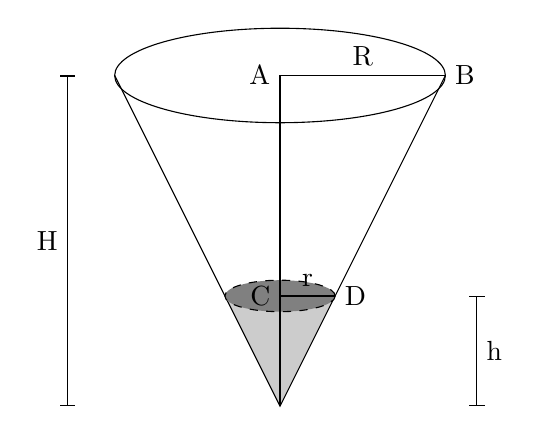
\begin{tikzpicture}
% 底部
\draw (0,0) ellipse (21mm and 6mm);
% 底部至截面的斜面
\draw (21mm,0) -- (7mm,-28mm);
\draw (-21mm,0) -- (-7mm,-28mm);
% 顶部至截面
\draw[fill=black!20] (-7mm,-28mm) -- (0,-42mm) -- (7mm,-28mm);
% 截面
\draw[dashed, fill=black!50] (0,-28mm) ellipse (7mm and 2mm);
% 高辅助线
\draw (0,0) -- (0, -42mm);
% 底部半径辅助线
\draw (0,0) node[left]{A} -- node[auto]{R} (21mm, 0) node[right]{B};
% 截面半径辅助线
\draw (0,-28mm) node[left]{C} -- node[auto]{r} (7mm,-28mm) node[right]{D};
% 高标识
\draw[|-|] (-27mm,0) -- node[auto, swap]{H} (-27mm,-42mm);
\draw[|-|] (25mm,-28mm) -- node[auto]{h} (25mm,-42mm);
\end{tikzpicture}
\end{document}
